\documentclass[12pt]{article}

\usepackage[utf8]{inputenc}
\usepackage[brazil]{babel}
\usepackage[margin=2.5cm]{geometry}
\usepackage{booktabs}
\usepackage{graphicx}
\usepackage{amsmath}
\usepackage{natbib}
\bibliographystyle{plainnat}

\title{Relatório de Análise da Variável Temperatura}
\author{Vinicius Lucio}
\date{\today}

\begin{document}

\maketitle

\section{Introdução e Descrição dos Dados}

Os dados analisados neste relatório foram obtidos do conjunto de dados clássico \texttt{airquality}, originário de medições diárias de qualidade do ar e variáveis meteorológicas em Nova York durante o período de maio a setembro de 1973 \citep{Chambers1983}. O arquivo contém 153 observações no total. A análise foca na variável \texttt{Temp} (temperatura diária medida em graus Fahrenheit às 07h00 no aeroporto LaGuardia), a qual apresenta zero valores ausentes (\texttt{NA}) ao longo de todo o monitoramento. As rotinas e manipulações computacionais foram conduzidas no ambiente estatístico R \citep{RCoreTeam}.

\section{Resumo Estatístico e Distribuição Mensal}

Para cada mês avaliado, a média aritmética da temperatura foi obtida por meio da equação \eqref{eq:media}:
\begin{equation}
\label{eq:media}
\bar{x}_m = \frac{1}{n_m} \sum_{i=1}^{n_m} x_{m,i}
\end{equation}
Na equação \eqref{eq:media}, o denominador $n_m$ contabiliza estritamente o número de dias efetivamente medidos no mês $m$, descartando observações com valores ausentes quando existirem. 

Os valores calculados a partir dos dados constam na Tabela~\ref{tab:resumo}. Observa-se um aumento progressivo da média térmica a partir de maio, atingindo o ápice nos meses de julho e agosto, seguido de um declínio em setembro.

\begin{table}[htbp]
\centering
\caption{Média da temperatura por mês e contagem de dias medidos (Nova York, 1973).}
\label{tab:resumo}
\begin{tabular}{ccc}
\toprule
Mês & Dias Medidos & Média ($^\circ\text{F}$) \\
\midrule
5 & 31 & 65.55 \\
6 & 30 & 79.10 \\
7 & 31 & 83.90 \\
8 & 31 & 83.97 \\
9 & 30 & 76.90 \\
\bottomrule
\end{tabular}
\end{table}

A distribuição completa e a dispersão dos valores ao longo de cada período podem ser visualizadas na Figura~\ref{fig:distribuicao}, gerada a partir do script correspondente.

\begin{figure}[htbp]
\centering
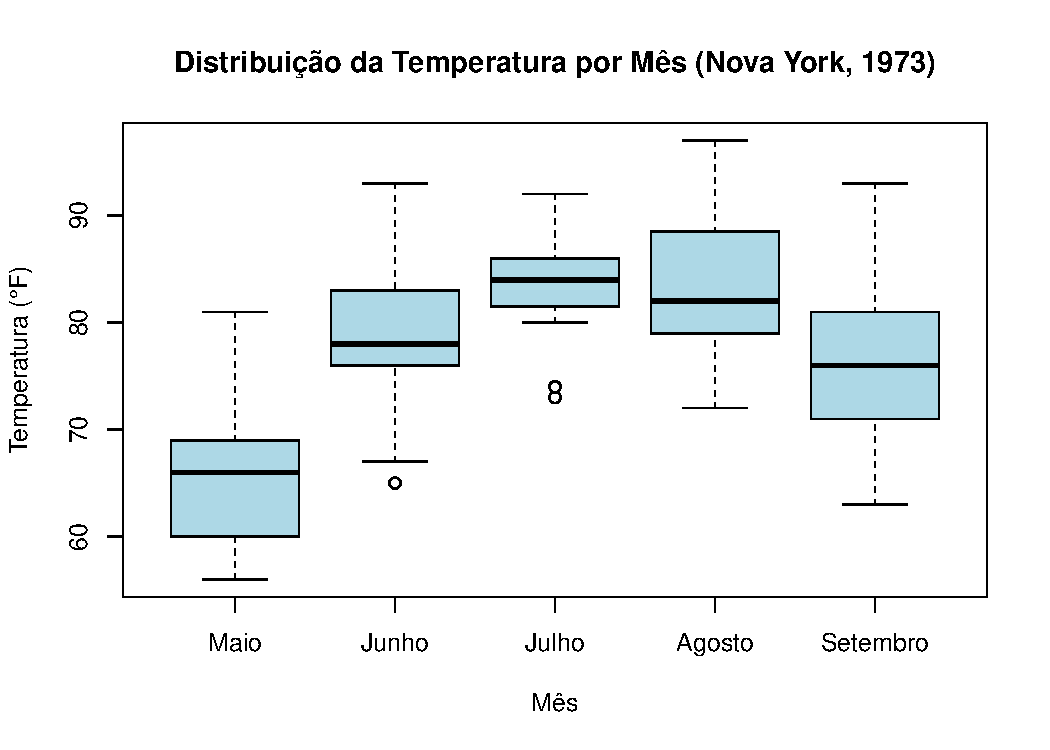
\includegraphics[width=0.75\textwidth]{figura.pdf}
\caption{Distribuição mensal da temperatura através de gráficos de caixas (\emph{boxplots}).}
\label{fig:distribuicao}
\end{figure}

\bibliography{referencias}

\end{document}
